\documentclass{beamer}
\usepackage[utf8]{inputenc}
\usepackage{graphicx, epsfig}
\usepackage{amsmath,mathrsfs,amsfonts,amssymb}
\usepackage{floatflt}
\usepackage{epic,ecltree}
\usepackage{mathtext}
\usepackage{fancybox}
\usepackage{fancyhdr}
\usepackage{multirow}
\usepackage{enumerate}
\usepackage{epstopdf}
\usepackage{multicol}
\usepackage{algorithm}
\usepackage[noend]{algorithmic}
\usepackage{tikz}
\usepackage{blindtext}
\usetheme{default}%{Singapore}%{Warsaw}%{Warsaw}%{Darmstadt}
\usecolortheme{default}

\setbeamerfont{title}{size=\Huge}
\setbeamertemplate{footline}[page number]{}

\setbeamertemplate{section in toc}[sections numbered]


\makeatletter
\newcommand\HUGE{\@setfontsize\Huge{35}{40}}
\makeatother    

\setbeamerfont{title}{size=\HUGE}
\beamertemplatenavigationsymbolsempty

% latin bold lower
\newcommand{\ba}{\mathbf{a}} 
\newcommand{\bc}{\mathbf{c}} 
\newcommand{\be}{\mathbf{e}} 
\newcommand{\bh}{\mathbf{h}} 
\newcommand{\bp}{\mathbf{p}} 
\newcommand{\bt}{\mathbf{t}} 
\newcommand{\bs}{\mathbf{s}} 
\newcommand{\bu}{\mathbf{u}} 
\newcommand{\bv}{\mathbf{v}} 
\newcommand{\bw}{\mathbf{w}} 
\newcommand{\bx}{\mathbf{x}} 
\newcommand{\by}{\mathbf{y}} 
\newcommand{\bz}{\mathbf{z}} 

% latin bold upper
\newcommand{\bA}{\mathbf{A}} 
\newcommand{\bB}{\mathbf{B}} 
\newcommand{\bC}{\mathbf{C}} 
\newcommand{\bI}{\mathbf{I}} 
\newcommand{\bJ}{\mathbf{J}} 
\newcommand{\bL}{\mathbf{L}} 
\newcommand{\bM}{\mathbf{M}} 
\newcommand{\bQ}{\mathbf{Q}} 
\newcommand{\bT}{\mathbf{T}} 
\newcommand{\bU}{\mathbf{U}} 
\newcommand{\bV}{\mathbf{V}} 
\newcommand{\bW}{\mathbf{W}} 
\newcommand{\bX}{\mathbf{X}} 
\newcommand{\bY}{\mathbf{Y}} 
\newcommand{\bZ}{\mathbf{Z}} 

% latin cal upper
\newcommand{\cG}{\mathcal{G}} 
\newcommand{\cL}{\mathcal{L}} 
\newcommand{\cN}{\mathcal{N}} 
\newcommand{\cS}{\mathcal{S}} 
\newcommand{\cT}{\mathcal{T}} 
\newcommand{\cW}{\mathcal{W}} 
\newcommand{\cX}{\mathcal{X}} 
\newcommand{\cZ}{\mathcal{Z}} 

% latin bb upper
\newcommand{\bbE}{\mathbb{E}} 
\newcommand{\bbI}{\mathbb{I}} 
\newcommand{\bbP}{\mathbb{P}} 
\newcommand{\bbR}{\mathbb{R}} 

% greek bold lower
\newcommand{\bepsilon}{\boldsymbol{\epsilon}} 
\newcommand{\btheta}{\boldsymbol{\theta}} 
\newcommand{\blambda}{\boldsymbol{\lambda}} 
\newcommand{\bpi}{\boldsymbol{\pi}} 
\newcommand{\bmu}{\boldsymbol{\mu}} 
\newcommand{\bsigma}{\boldsymbol{\sigma}} 
\newcommand{\bphi}{\boldsymbol{\phi}} 

% greek bold upper
\newcommand{\bSigma}{\boldsymbol{\Sigma}} 

\DeclareMathOperator*{\argmin}{arg\,min}
\DeclareMathOperator*{\argmax}{arg\,max}

\newcommand{\createdgmtitle}[1]{\title[\hbox to 56mm{Deep Learning Audio \hfill\insertframenumber\,/\,\inserttotalframenumber}]
	{\vspace{1cm} \\ Deep Learning Audio \\ {\Huge Lecture #1}}
	\author{Pavel Severilov}
	\institute{
	Moscow Institute of Physics and Technology
	} 
	\date{2022}
}

\newcommand\myfootnote[1]{%
  \tikz[remember picture,overlay]
  \draw (current page.south west) +(1in + \oddsidemargin,0.5em)
  node[anchor=south west,inner sep=0pt]{\parbox{\textwidth}{%
      \rlap{\rule{10em}{0.4pt}}\raggedright\scriptsize \textit{#1}}};}

\newcommand\myfootnotewithlink[2]{%
  \tikz[remember picture,overlay]
  \draw (current page.south west) +(1in + \oddsidemargin,0.5em)
  node[anchor=south west,inner sep=0pt]{\parbox{\textwidth}{%
      \rlap{\rule{10em}{0.4pt}}\raggedright\scriptsize\href{#1}{\textit{#2}}}};}
      
\AtBeginSection[]
{
	\begin{frame}{Outline}
		\tableofcontents[currentsection,subsectionstyle=hide]
	\end{frame}
}
\AtBeginSubsection[]{
	\begin{frame}{Outline}
		\tableofcontents[currentsection,currentsubsection]
	\end{frame}
}
\createdgmtitle{1}
\usepackage{tikz}
\usetikzlibrary{arrows,shapes,positioning,shadows,trees}
%--------------------------------------------------------------------------------
\begin{document}
%--------------------------------------------------------------------------------
\begin{frame}[noframenumbering,plain]
%\thispagestyle{empty}
\titlepage
\end{frame}
%=======x
\begin{frame}{Outline}
	\tableofcontents
\end{frame}
%=======
\section{Organisation}
%=======
\begin{frame}{Organisation}
	\begin{enumerate}
		\item $\sim 7$ lectures
		\item 2 homeworks
		\item Grade: 
		\begin{itemize}
			\item 50\% homeworks + 50\%  one exam question
			\item or 100\% your project
		\end{itemize}
		\item Github course page: slides+videos+homeworks+materials+papers \url{https://github.com/severilov/2022-DL-Audio-Course}
		\item Discussion: telegram chat (contact @severilov)
		%\item ? Maybe seminars
	\end{enumerate}
\end{frame}
%=======
\section{Tasks}
%=======
\begin{frame}{Voice Technologies: Applications}
	\begin{figure}
		\centering
		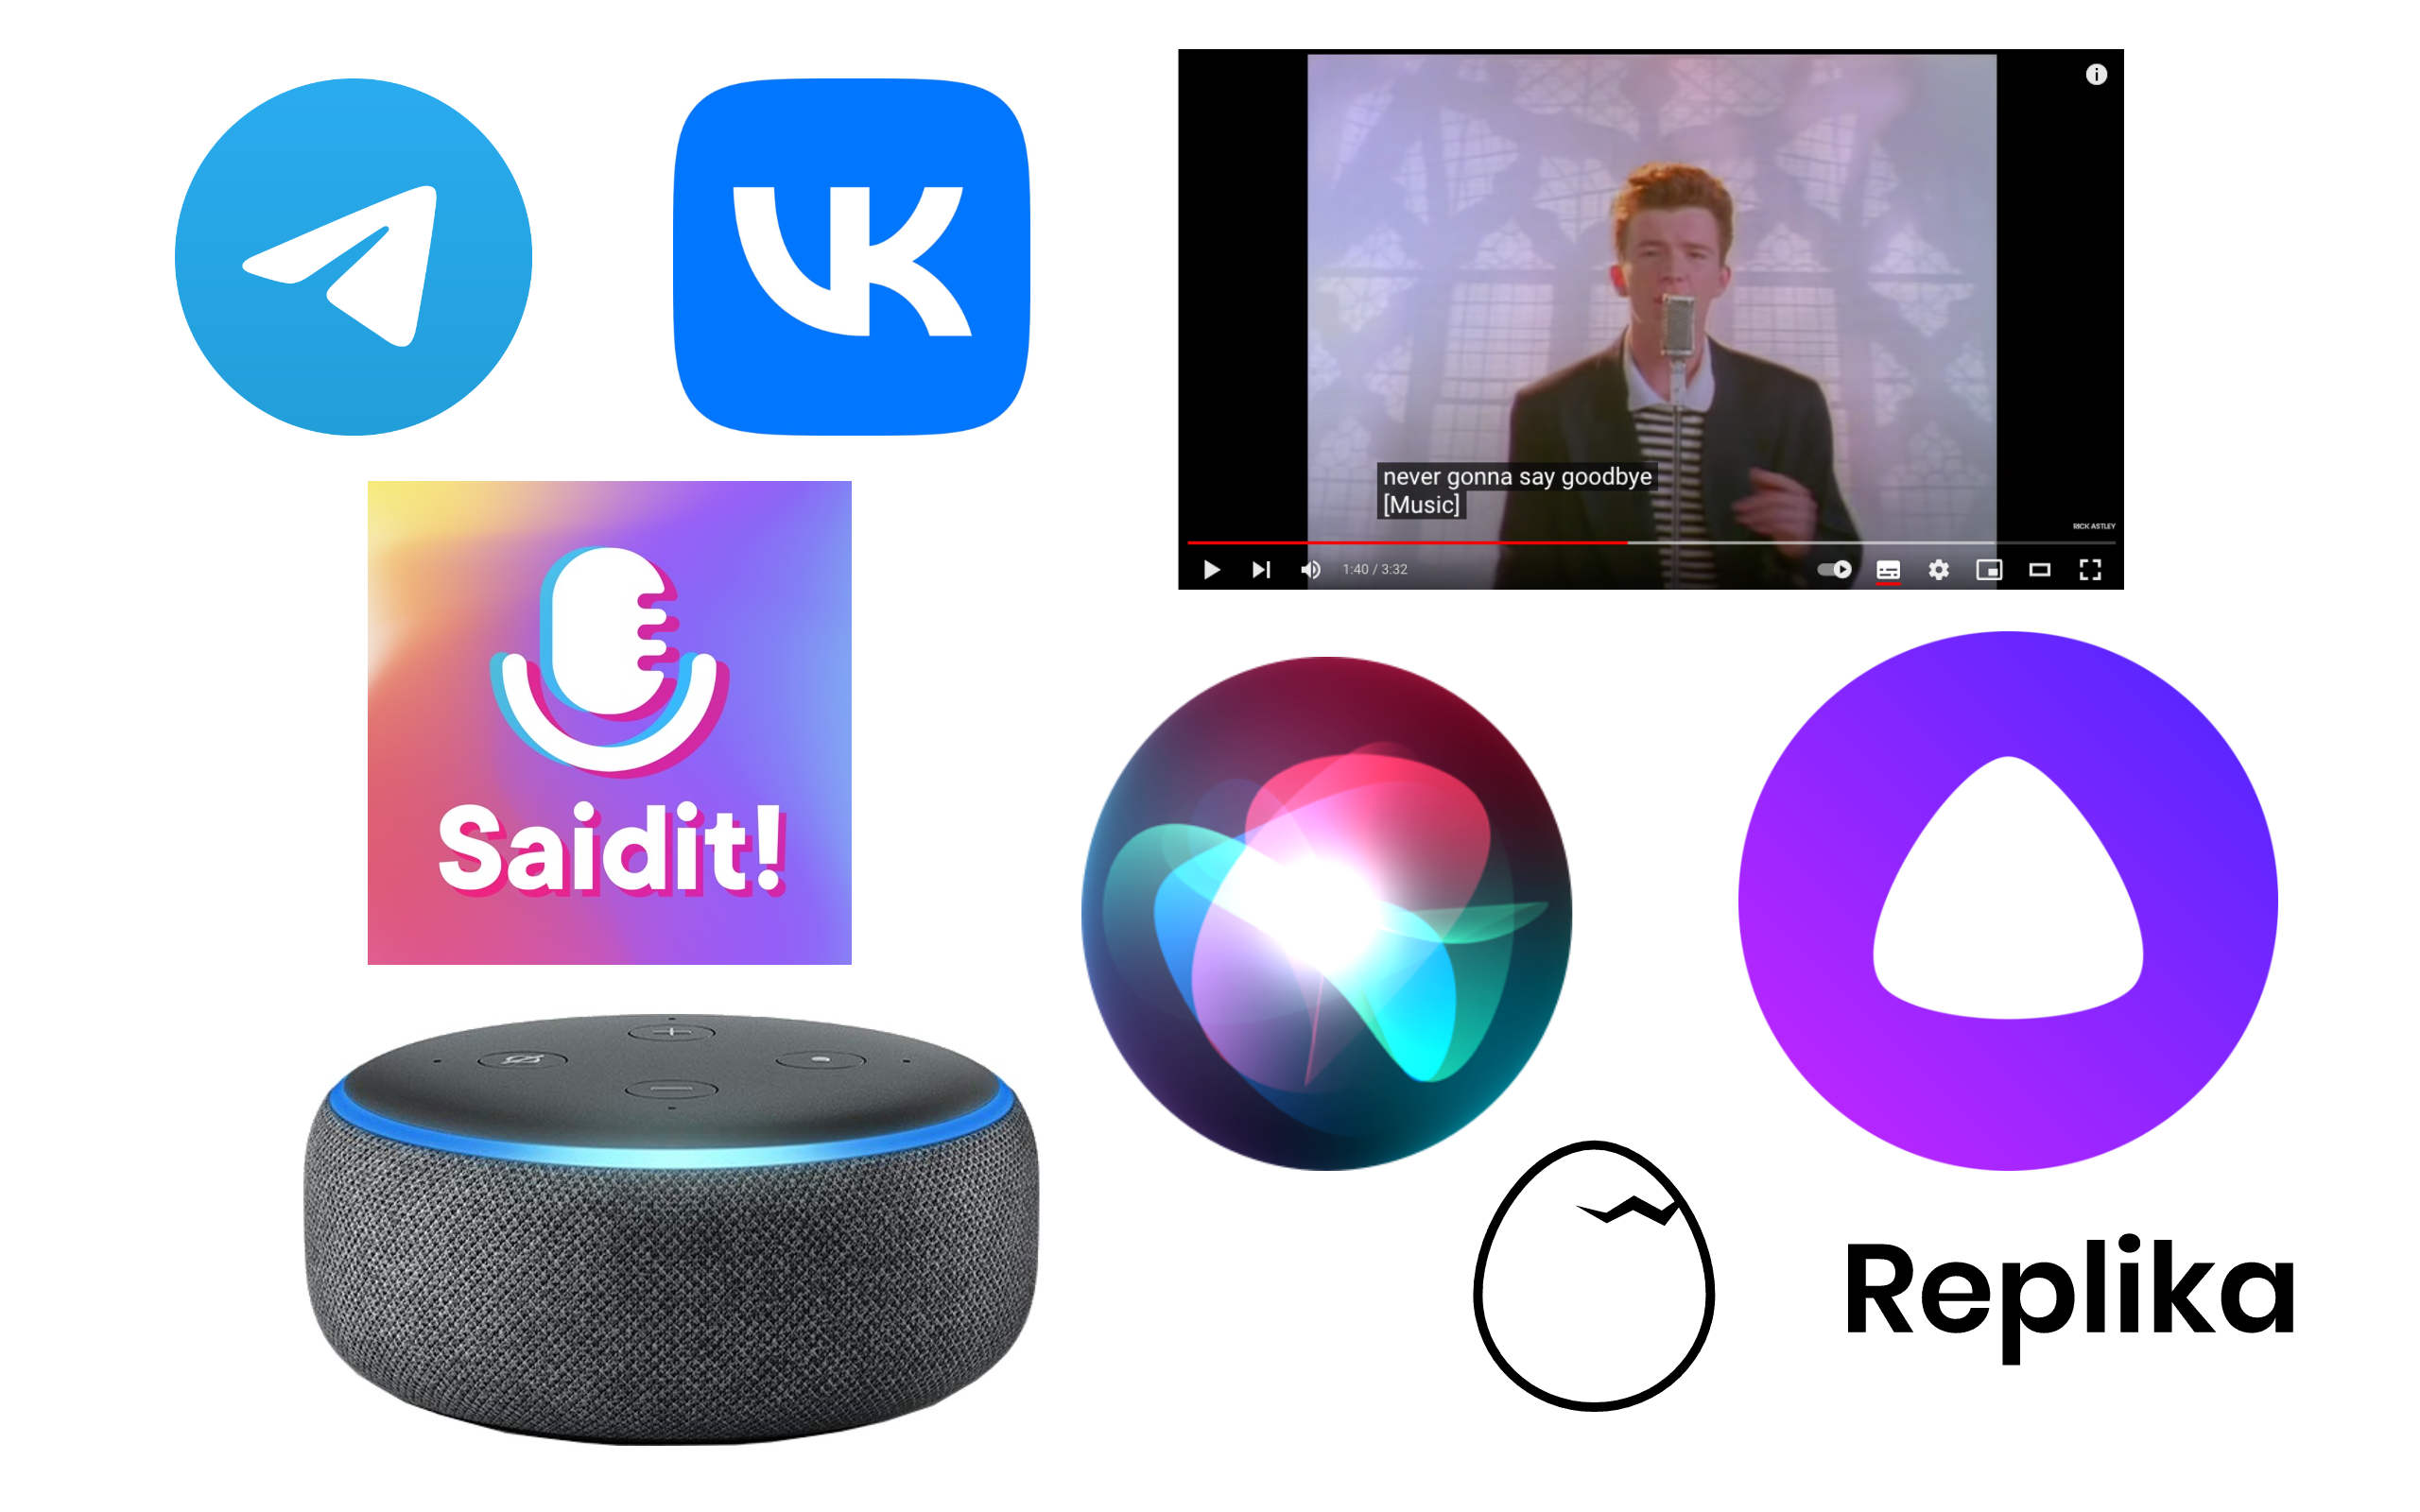
\includegraphics[width=0.99\linewidth]{figs/applications.png}
		\caption{Siri, Amazon Alexa, Alisa, Replika, Telegram, VK, YouTube}
	\end{figure}
\end{frame}
%=======
\begin{frame}{Voice Technologies, Tasks: Mind Map}
	\begin{figure}
		\centering
		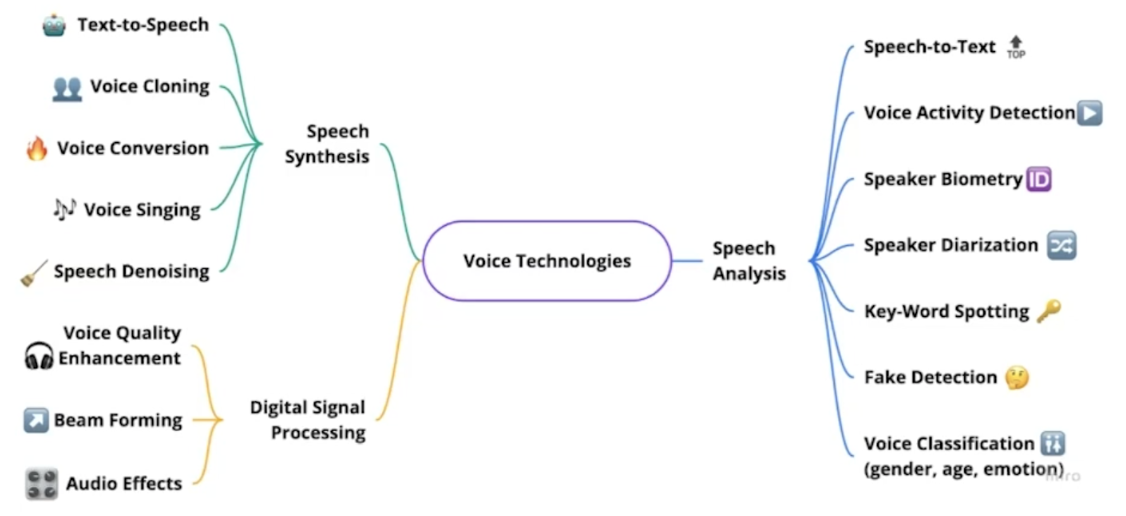
\includegraphics[width=1.03\linewidth]{figs/tasks_1.png}
	\end{figure}
	\myfootnotewithlink{https://github.com/yandexdataschool/speech\_course}{Yandex School of Data Analysis, Speech Processing Course}
\end{frame}
%=======
\begin{frame}{Voice Technologies, Tasks: Course}
	\begin{figure}
		\centering
		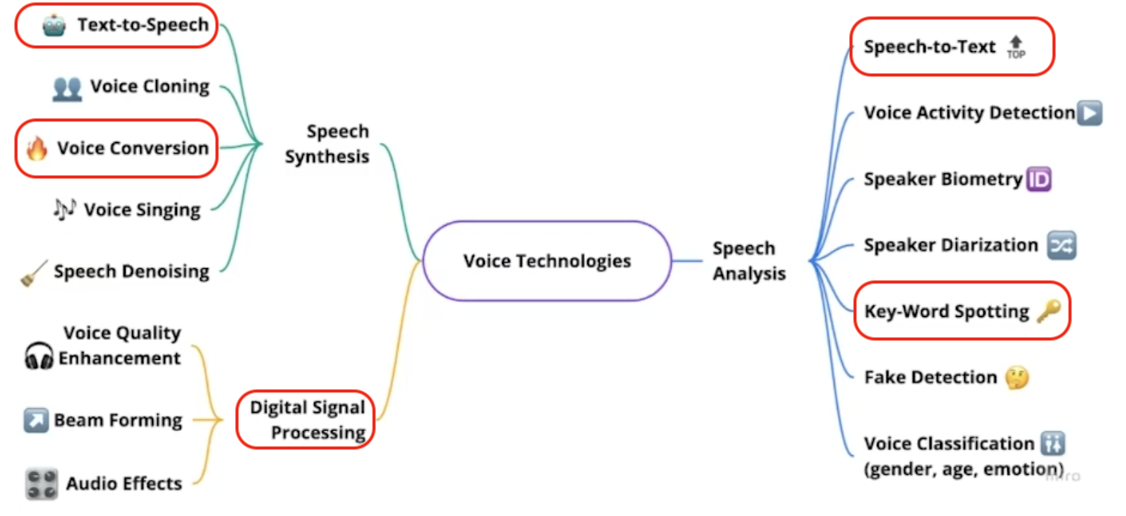
\includegraphics[width=1.03\linewidth]{figs/tasks_1_course.png}
	\end{figure}
\end{frame}
%=======

\section{Speech Recognition}
%=======
\begin{frame}{History of Speech Recognition}
	\begin{figure}
		\centering
		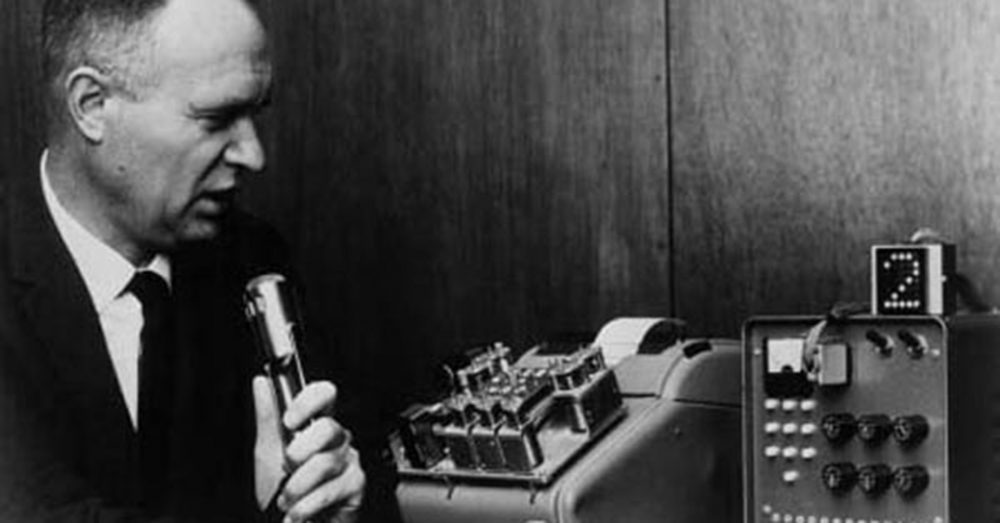
\includegraphics[width=0.7\linewidth]{figs/audrey.png}
	\end{figure}
	\begin{itemize}
		\item \textbf{50's}: 1952, Bell Laboratories, "Audrey" system, could recognize single voice speking digits
		\item \textbf{60's}: 1961, IBM, "Shoebox", understood 16 words in English
		\item \textbf{70's}: DARPA, understood over 1000 words (Siri spin-out)
		\item \textbf{80's}: using HMM, understood several thousand words
		\item \textbf{90's}: became faster because of processors
		\item \textbf{00's-10's}: ML, DL, Big Data, GPUs
	\end{itemize}
\end{frame}
%=======
\begin{frame}{Speech Analysis Tasks: Mind Map}
	\begin{figure}
		\centering
		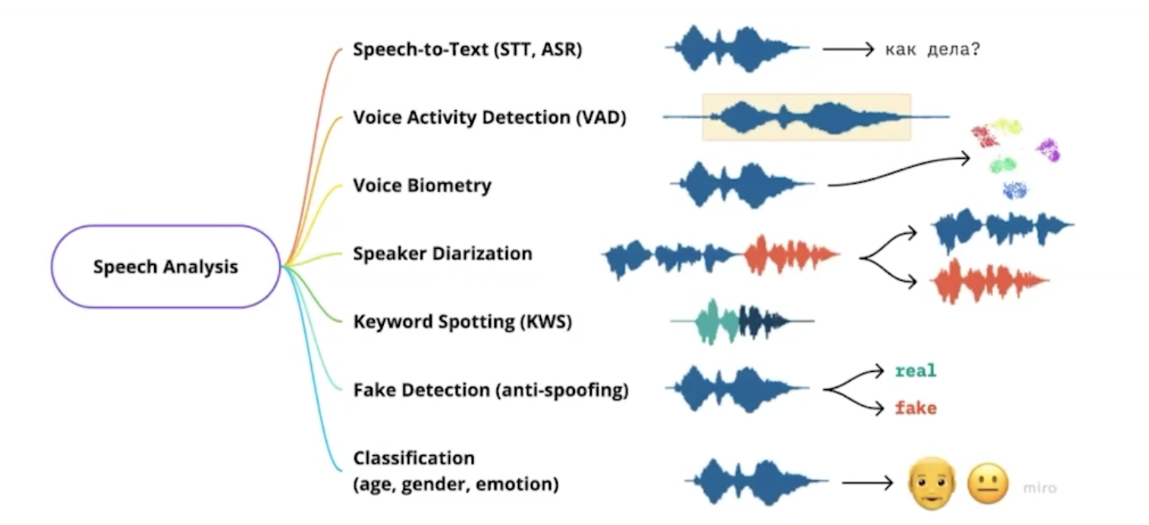
\includegraphics[width=0.99\linewidth]{figs/tasks_2.png}
	\end{figure}
	\myfootnotewithlink{https://github.com/yandexdataschool/speech\_course}{Yandex School of Data Analysis, Speech Processing Course}
\end{frame}
%=======
\begin{frame}{Speech Recognition \& Deep Learning: Idea}
	\begin{figure}
		\centering
		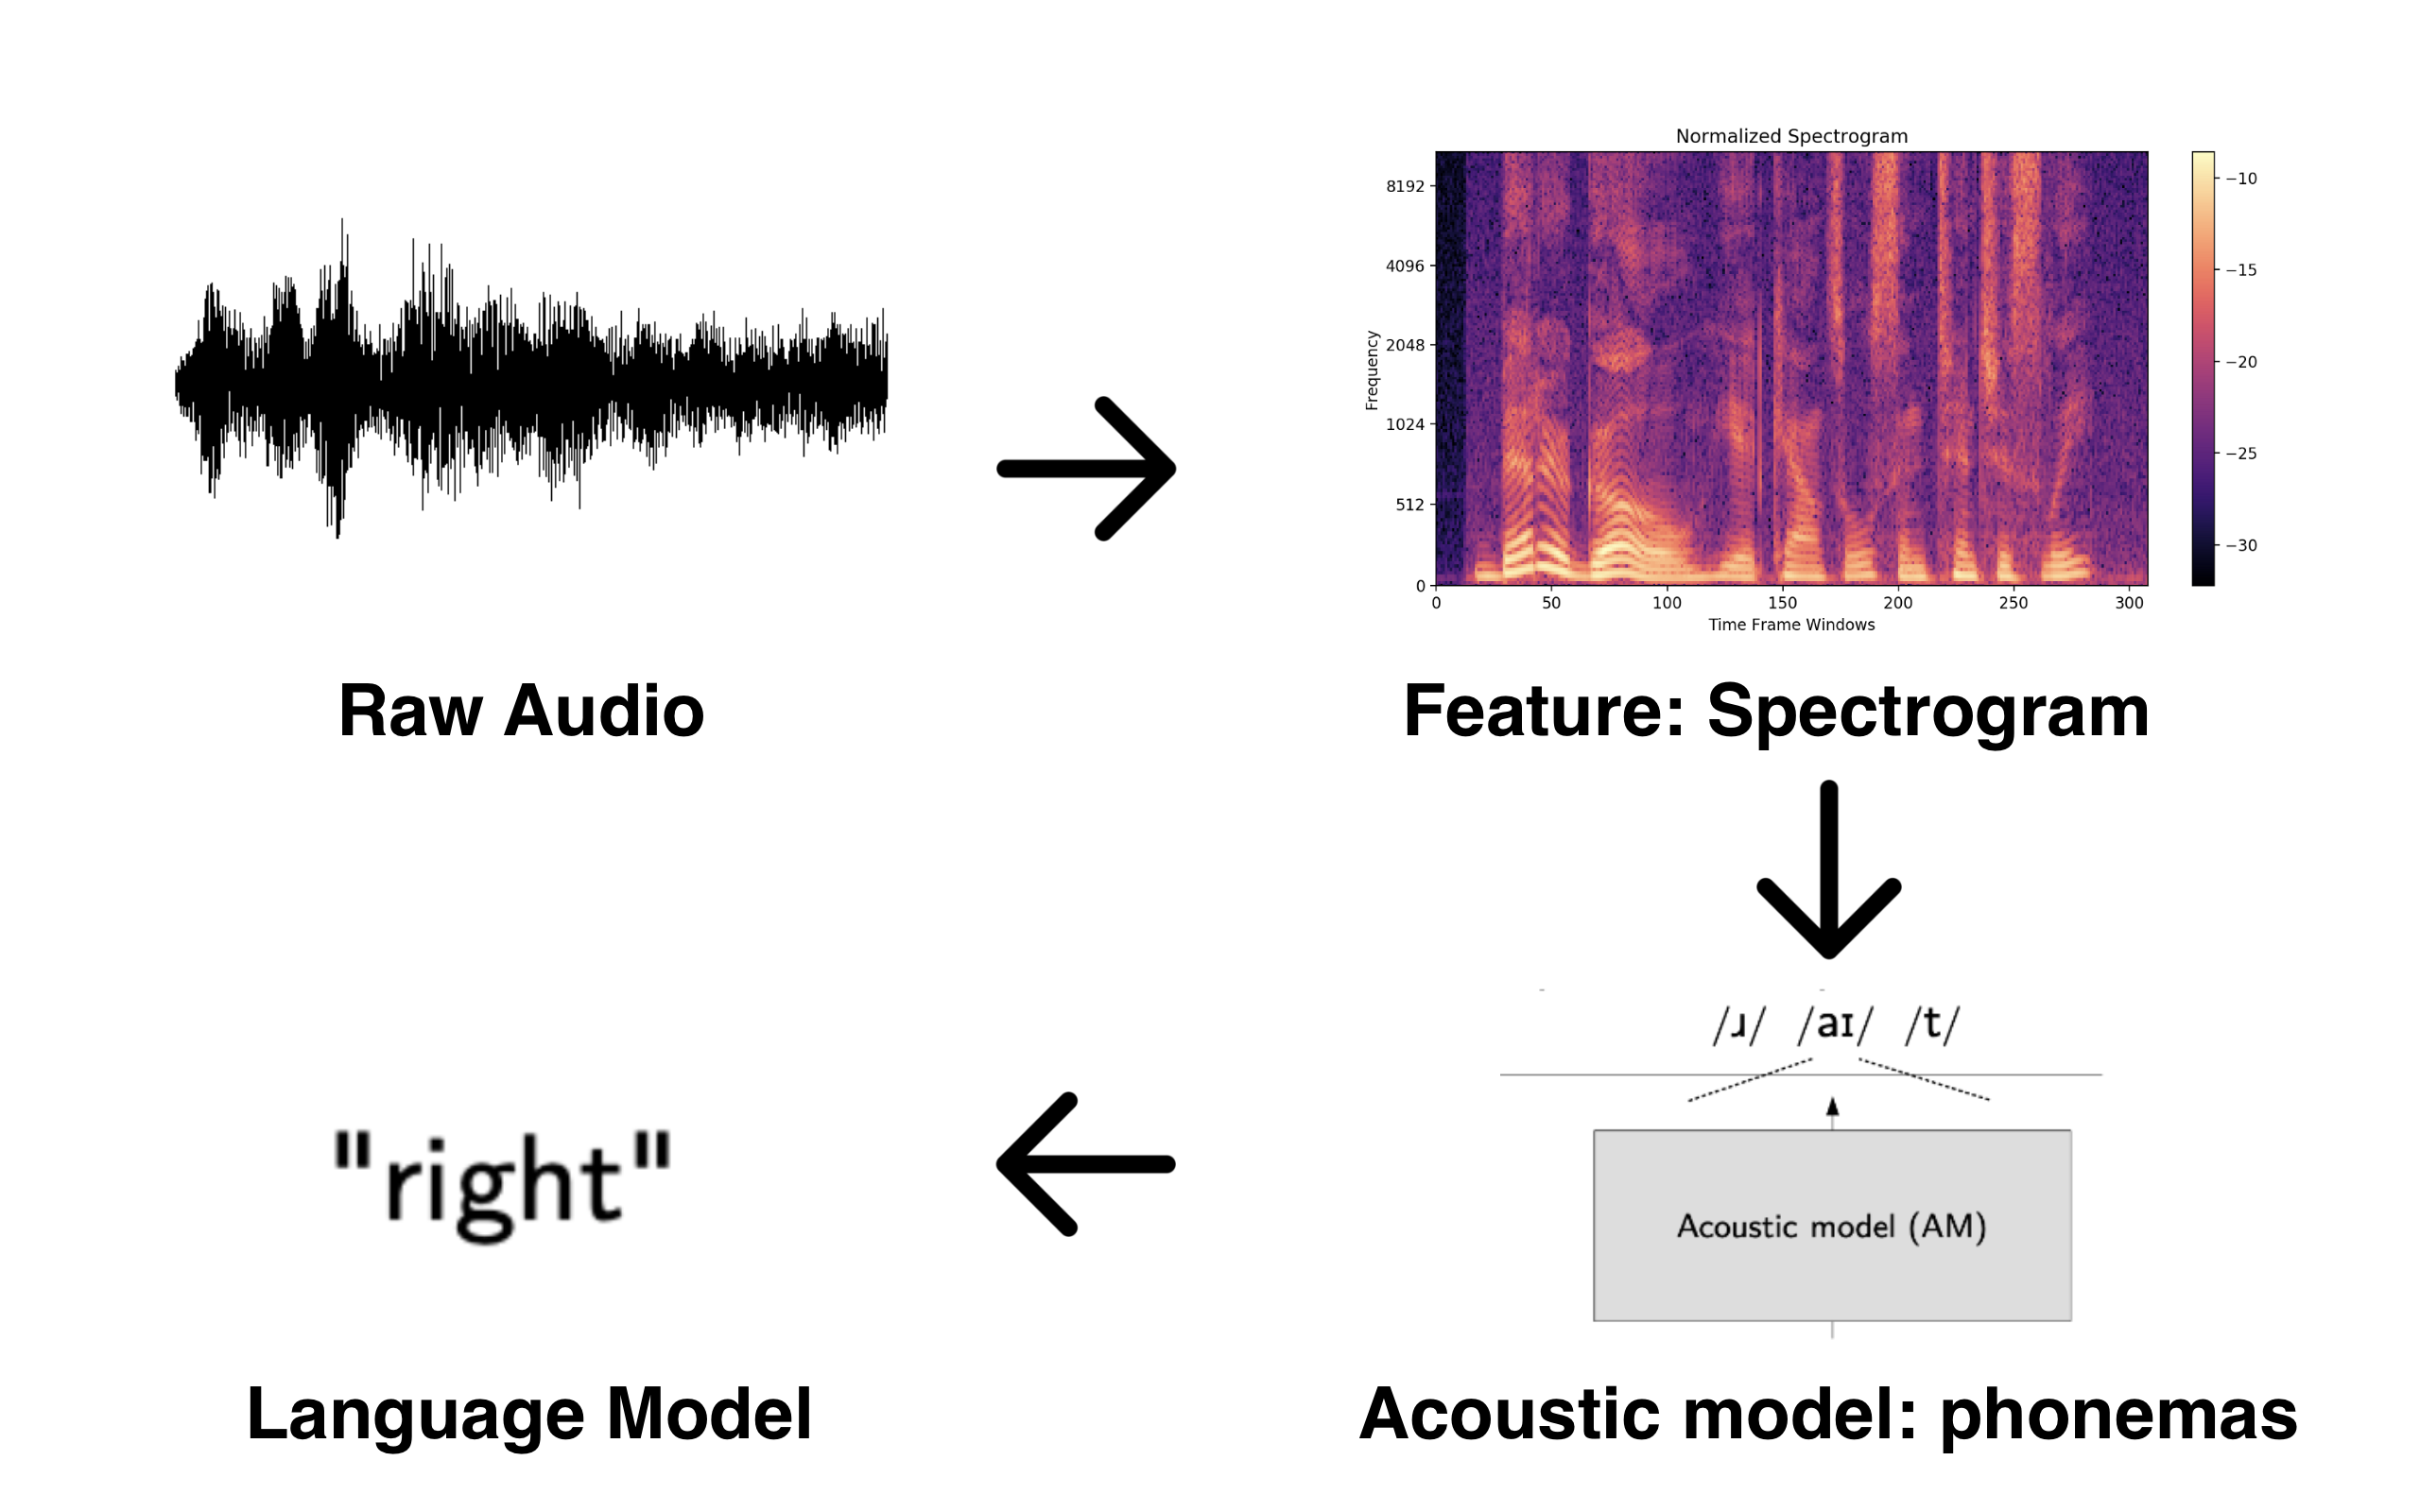
\includegraphics[width=0.99\linewidth]{figs/asr.png}
	\end{figure}
\end{frame}
%=======
%=======
\section{Speech Synthesis}
%=======
\begin{frame}{History of Speech Synthesis}
	\begin{figure}
		\centering
		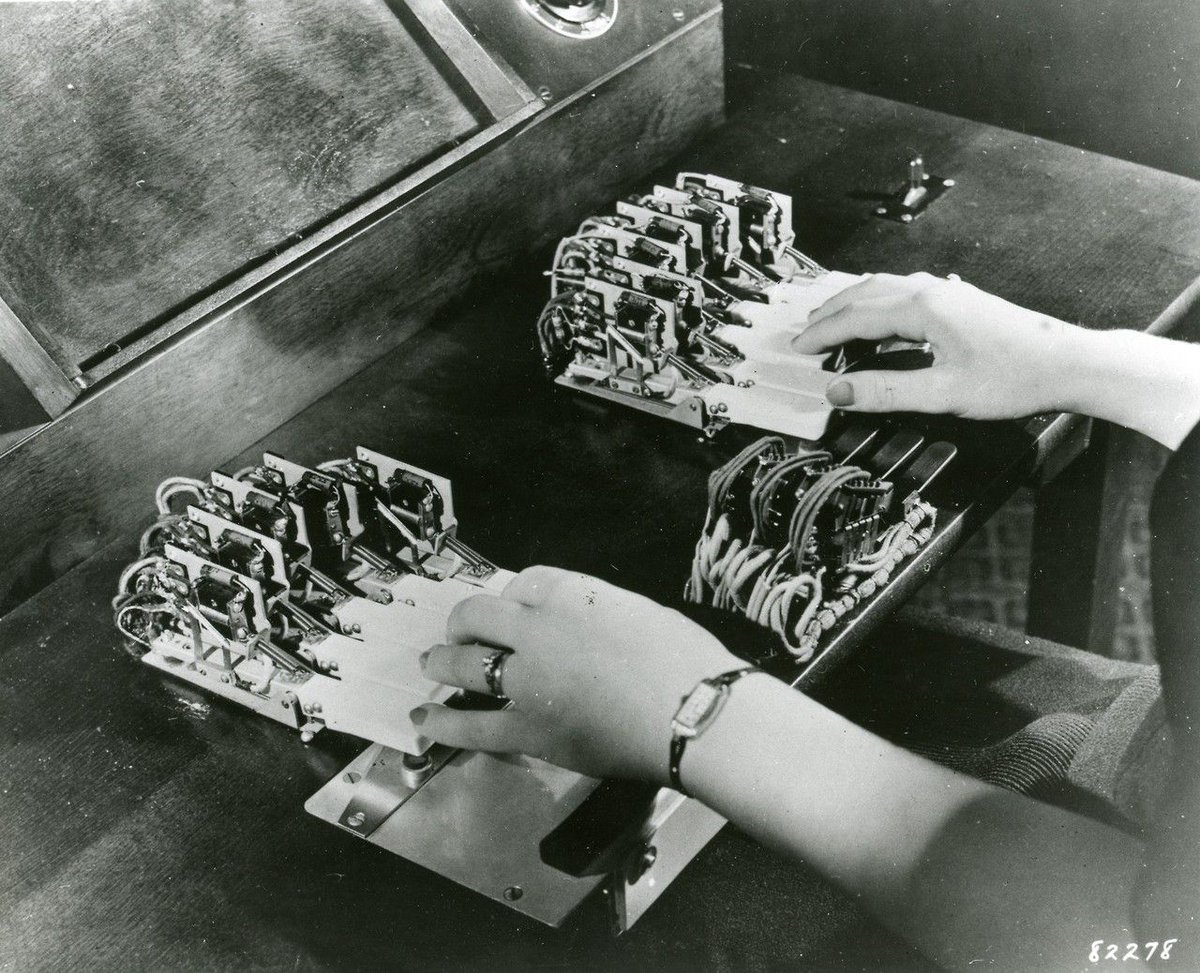
\includegraphics[width=0.6\linewidth]{figs/voder.png}
	\end{figure}
	\begin{itemize}
		\item \textbf{30's}: 1939, Bell Laboratories, "Voder",
		\item \textbf{80's}: Format-based on rules, Atari/Sega
		\item \textbf{90's-00's}: Concatenative synthesis
		\item \textbf{10's}: ML, DL, Big Data, GPUs
	\end{itemize}
\end{frame}
%=======
\begin{frame}{Speech Synthesis Tasks: Mind Map}
	\begin{figure}
		\centering
		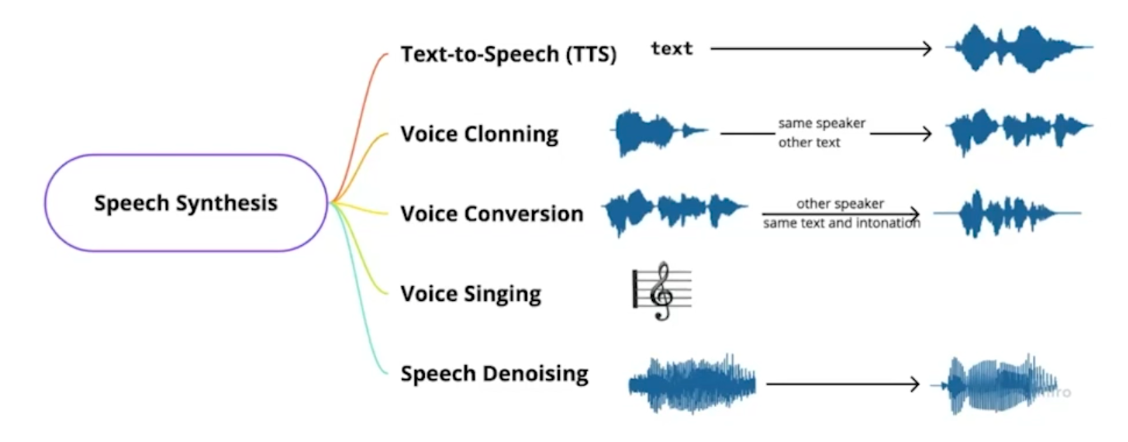
\includegraphics[width=0.99\linewidth]{figs/tasks_3.png}
	\end{figure}
	\myfootnotewithlink{https://github.com/yandexdataschool/speech\_course}{Yandex School of Data Analysis, Speech Processing Course}
\end{frame}
%=======
\begin{frame}{Speech Synthesis \& Deep Learning: Idea}
	\begin{figure}
		\centering
		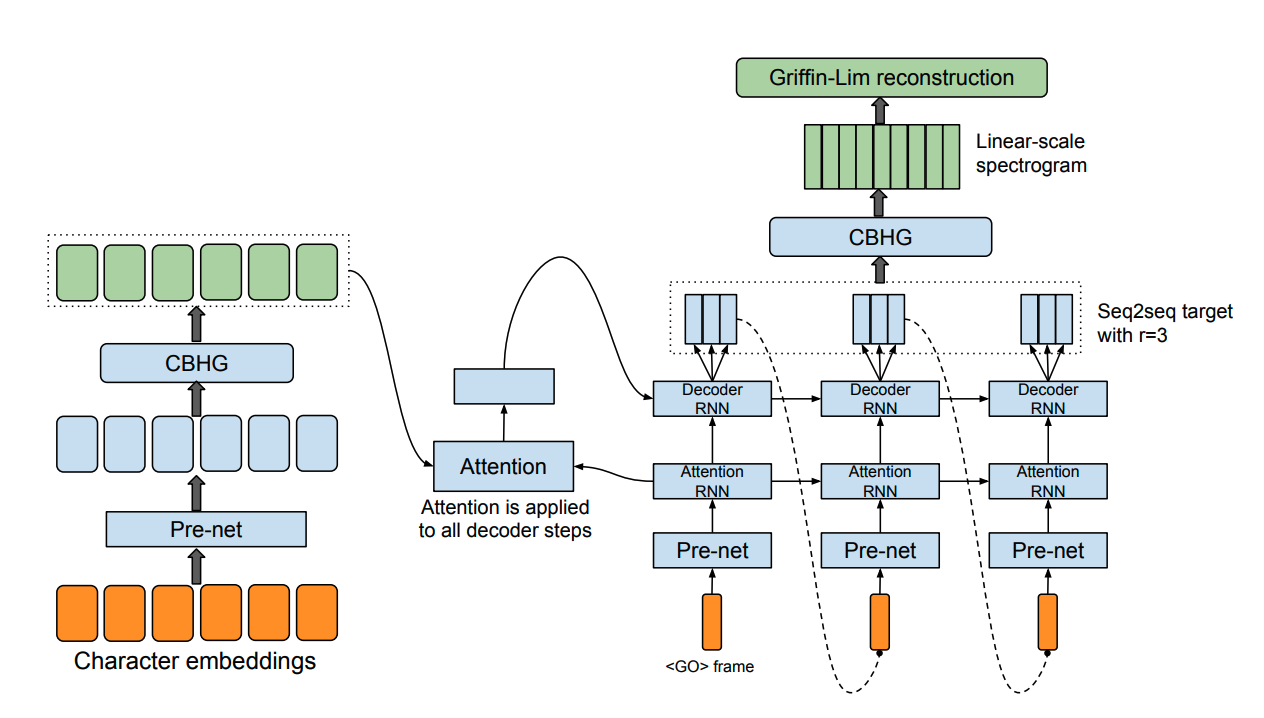
\includegraphics[width=0.99\linewidth]{figs/tts.png}
		\caption{Example of Deep Learning approach to speech synthesis: encoder-decoder structure with reccurent parts}
	\end{figure}
	\myfootnotewithlink{https://arxiv.org/abs/1703.10135}{Wang, Yuxuan et al. “Tacotron: Towards End-to-End Speech Synthesis.” INTERSPEECH (2017), Google Inc.}
\end{frame}
%=======
\end{document} 